\documentclass[a4paper,12pt]{article}
\usepackage[utf8]{inputenc}
\usepackage[T1]{fontenc}
\usepackage[hungarian]{babel}
\usepackage{graphicx}
\usepackage{geometry}
\geometry{a4paper,
		     tmargin = 35mm, 
		     lmargin = 25mm,
		     rmargin = 30mm,
		     bmargin = 30mm}
\usepackage{mathtools}
\usepackage{amsmath}
\usepackage{color}
\usepackage{setspace}
\usepackage{amsmath,amssymb}
\usepackage{float}


\usepackage{indentfirst}
\usepackage{subfig}

\renewcommand\thesection{\Roman{section}}

\begin{document}

\linespread{1.2}

\begin{titlepage}

	\centering
	
\includegraphics[width=0.66\textwidth]{elte.jpg}\par\vspace{1cm}
	{\scshape\LARGE ELTE TTK \par}
	\vspace{3cm}
	{\scshape\Large Az Compton-effektus vizsgálata\par}
	\vspace{1cm}
	{\large\itshape Olar Alex\par}
	\vspace{3cm}
	laborvezető\par
	\vspace{0.3cm}
	{\Large Csanád Máté}
	\vfill
	{\large 2018 \par}
	
\end{titlepage}

\begin{abstract}
\par A mérés célja az volt, hogy a kiértékelés során a lehető legpontosabban járjunk el a számolások közben, hibabecslésen alkalmával. A Compton-effektus tulajdonságait vizsgáltuk. Az energia és a hatáskereszmetszet elméleti szögfüggését vettük alapul a kiértékelés során.
\end{abstract}

\vfill

\tableofcontents

\newpage

\section{Mérési eszközök}

\begin{itemize}
\item plasztik elektron detektor
\item állítható fotodetektor
\item sokcsatornás analizátor (MCA)
\item számítógép
\item $^{137}Cs$, közvetett $\gamma$-foton forrás
\end{itemize}

\subsection{Mérési elrendezés}

\par A mérési elrendezésről néhány kép, ahonnan a felhasznált adatokat vettük.

\vspace{1cm}

\begin{figure}[!htb]
\centering
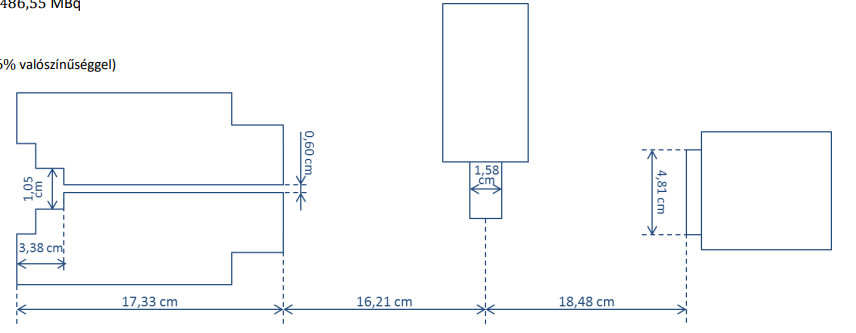
\includegraphics[width=0.86\textwidth]{meresi.png}
\end{figure}

\section{Elméleti összefoglaló}

\par A Compton-effektus a fotonok, lazán kötött (kvázi szabad) elektronokon való szóródását írja le, alapegyenlete a négyesimpulzus megmaradásból következik

\begin{equation*}
	E = \frac{E_{0}}{1 + \frac{E_{0}}{m_{e}c^{2}}(1 - cos\vartheta)}	
\end{equation*}

ahol $\vartheta$ az foton szórási szögét, $E_{0}$ annak kezdeti energiáját, míg $m_{e}$ az elektron tömegét jelöli. A mérés során $E_{0}$ értéke adott, a $\gamma$-fotonok $662~keV$ enerigával rendelkeznek. Természetesen $E$ a szórt fotonok energiáját jelöli.
\par Bevezetve a $P = \frac{E}{E_{0}}$ arányszámot, az elméleti differenciális hatáskeresztmetszet felírható

\begin{equation*}
	\frac{d\sigma}{d\Omega} = \frac{1}{2}r_{0}^{2}(P - P^{2}sin^{2}\vartheta + P^{3})
\end{equation*}

alakban. Ahol $r_{0}$ a klasszikus elektronsugár, melynek értéke a Bohr-modell alapján számolható

\begin{equation*}
	r_{0} = \frac{1}{4\pi\epsilon_{0}}\frac{e^{2}}{m_{e}c^{2}} = 2.82 \times 10^{-15} ~m
\end{equation*}

\par A mérés során ezeket az összefüggéseket próbáljuk a lehető legpontosabban belátni.

\section{Mérési feladatok, kiértékelés}

\subsection{Aktivitás, dózis}

\par A $^{137}Cs$ minta aktivitása 1963. július 1-jén $486.55~MBq$ volt. A cézium felezési ideje $T = (11018 \pm 9.5)~nap$, míg az adott dátum óta eltelt napok száma a mérés időpontjáig $19 960~nap$ volt. Így az exponenciális bomlástörvény szerint, ma az aktivitás

\begin{equation*}
	A(t) = A_{0}2^{-\frac{t}{T}} = (138.61 \pm 0.08)~MBq
\end{equation*}

\par Mivel az elbomlott céziumokból további bomlás után nagyjából $94\%$-os valószínűséggel lesz $662~keV$-os $\gamma$-foton, így a másodpercenként közvetített teljes energia

\begin{equation*}
	\dot{E} = A(t)\eta E_{\gamma} = 1.38 \times 10^{-5} ~\frac{J}{s} 
\end{equation*}

amiből személyenként kapjuk az elnyelt dózist rendre akkor ha lenyeljük, 1 méterre vagyunk a forrástól, valamint ha 1 méterre, ólom árnyékolás választ el a forrástól

\begin{center}
\begin{tabular}{|c|c|c|}
\hline
dózis [mSv] - Dávid & dózis [mSv] - Marci & dózis [mSv] - Alex \\
\hline
3.15 & 2.25 & 2.4 \\
\hline
0.13 & 0.09 & 0.09 \\
\hline
5.69e-06 & 4.08e-06 & 4.27e-06 \\
\hline
\end{tabular}
\end{center}

ahol a mérés idejét 4 órának vettem és ezt helyettesíttem az adott képletekre melyek rendere

\begin{gather*}
D_{max} = \frac{\dot{E}\times 4\times 60\times 60}{m} \\
D_{1m} = \frac{\dot{E}\times 4\times 60\times 60}{m} \frac{0.5}{4\times 1^{2} \pi} \\
D_{1m, Pb} = \frac{\dot{E}\times 4\times 60\times 60}{m} \frac{0.5}{4\times 1^{2} \pi} \times e^{-10}
\end{gather*}

\par Látható, hogy árnyékolással és megfelelő távolságtartással nem számottevő a labor alatt elnyelt dózis, azonban ha közvetlenül a szerezetbe kerülne, már számottevő többlet dózist lehetne kapni.

\par Feladat volt még megbecsülni a $\vartheta = 0^{\circ}$ szögben, az elektron detektorra érkező fotonok számát másodpercenként. Ehhez felhasználva a mérési összeállítás geometriáját

\begin{equation*}
	N_{(foton, \vartheta = 0^{\circ})} = \frac{0.3^{2}}{4(17.33-3.38)^{2}}\times 138.61 ~(MBq) \times 1 ~(s) \approx 16 000
\end{equation*} 

\par Azonban ezalatt a mérés során ehhez kapcsolódóan nem volt több feladatunk.

\subsection{Szögfüggés vizsgálata}

\par A szögfüggéshez tartozó sokcsatornás beütésszámlálóval 10 különböző szöget vizsgáltunk mindegyiknék nagyjából $1000~s$-ig. Harminc fokról indulva, száztíz fokig néztük meg a beütésket, majd a hisztogrammokra exponenciális háttérrel, a Compton-csúcsra Gauss-görbét illesztettünk. Az illesztett adatok táblázatba foglalva

\begin{center}
\begin{tabular}{|c|c|c|c|c|c|c|c|}
\hline
szög [$^{\circ}$] & csatorna & szórás & terület & csatorna hiba & szórás hiba & terület hiba & idõ [t] \\
\hline
30 & 89.73 & 3.23 & 166 & 0.37 & 0.23 & 12 & 1224 \\
\hline
40 & 82.31 & 3.11 & 173 & 0.36& 0.44 & 35 & 1085 \\
\hline
50 & 74.37 & 2.43 & 120 & 0.42 & 0.27 & 13 & 1002 \\
\hline
60 & 66.15 & 1.96 & 85 & 0.43 & 0.43 & 26 & 962 \\
\hline
70 & 60.63 & 1.93 & 108 & 0.24 & 0.23 & 15 & 1166 \\
\hline
80 & 54.49 & 2.31 & 121 & 0.33 & 0.20 & 11 & 1100 \\
\hline
90 & 50.92 & 1.67 & 100 & 0.38 & 0.27 & 18 & 977 \\
\hline
100 & 46.62 & 1.46 & 101 & 0.19 & 0.13 & 9 & 1113 \\
\hline
110 & 42.88 & 1.82 & 155 & 0.34 & 0.31 & 44 & 1098 \\
\hline

\end{tabular}
\end{center}

\par A görbéket a $matplotlib$ könyvtárral illesztettük exponenciális háttérrel, amely paramétreit itt nem tűntettük fel. Az ábrák a kövekezőképpen festenek

\begin{figure}[!htb]
    \centering
    \begin{minipage}{.49\textwidth}
        \centering
        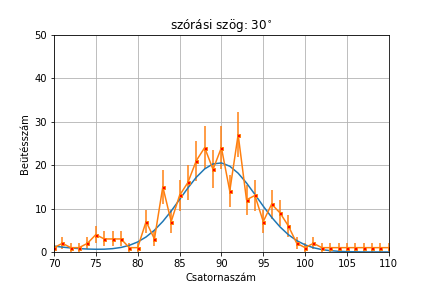
\includegraphics[width=1.\linewidth]{../plots/withbackground/30_1224fit.png}
    \end{minipage}
    \begin{minipage}{.49\textwidth}
        \centering
        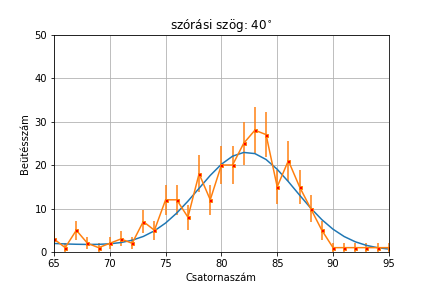
\includegraphics[width=1.\linewidth]{../plots/withbackground/40_1085fit.png}
    \end{minipage}
\end{figure}
\begin{figure}[!htb]
    \begin{minipage}{.49\textwidth}
        \centering
        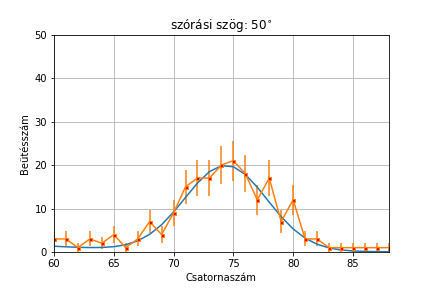
\includegraphics[width=1.\linewidth]{../plots/withbackground/50_1002fit.png}
    \end{minipage}%
    \begin{minipage}{.49\textwidth}
        \centering
        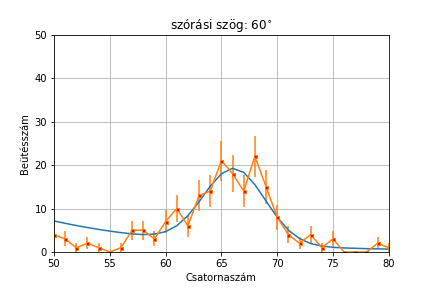
\includegraphics[width=1.\linewidth]{../plots/withbackground/60_962fit.png}
    \end{minipage}
    \begin{minipage}{.49\textwidth}
        \centering
        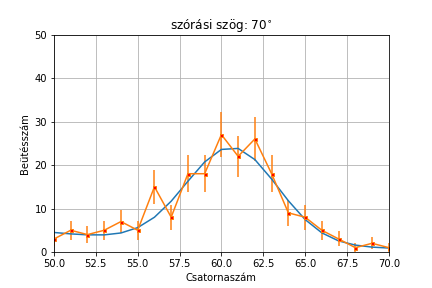
\includegraphics[width=1.\linewidth]{../plots/withbackground/70_1166fit.png}
    \end{minipage}%
    \begin{minipage}{.49\textwidth}
        \centering
        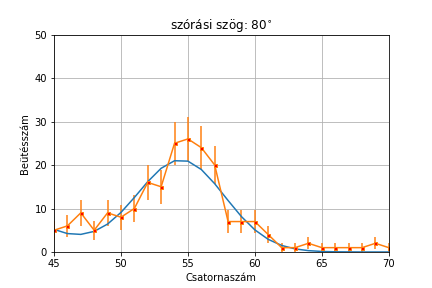
\includegraphics[width=1.\linewidth]{../plots/withbackground/80_1100fit.png}
    \end{minipage}
    \begin{minipage}{.49\textwidth}
        \centering
        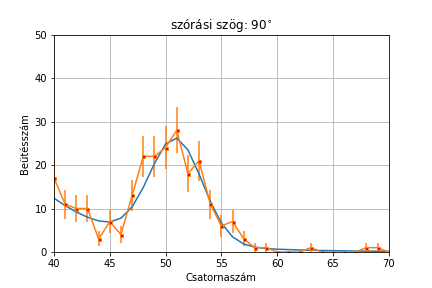
\includegraphics[width=1.\linewidth]{../plots/withbackground/90_977fit.png}
    \end{minipage}
    \begin{minipage}{.49\textwidth}
        \centering
        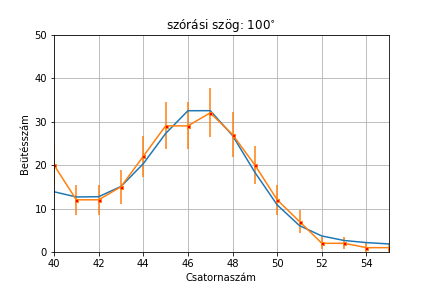
\includegraphics[width=1.\linewidth]{../plots/withbackground/100_1113fit.png}
    \end{minipage}
    \begin{minipage}{.49\textwidth}
        \centering
        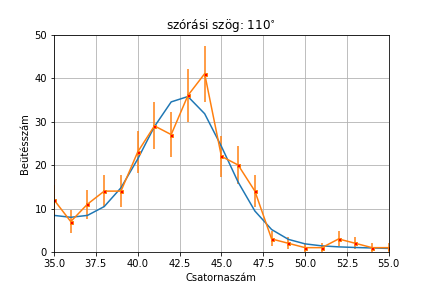
\includegraphics[width=1.\linewidth]{../plots/withbackground/110_1098fit.png}
    \end{minipage}
\end{figure}

\newpage

\par Az illesztés szisztematikus hibájának számításához 23 esetet néztünk végig. Az illesztés alsó szélétől és felső szélétől $\pm 5$ és a két legszélső helyzetet. Ezt csak a $110^{\circ}$-os esetre vizsgáltuk, a feltevés az, hogy a többi illesztés is ugyan ilyen relatív hibával rendelkezik.

\begin{center}
\begin{tabular}{|c|c|c|c|}
\hline
- & átlag & hiba (szórás) & relatív hiba [$\%$] \\
\hline
csatorna & 42.81 & 0.002 & 4.6$\times 10{-5}$ \\
\hline
szélesség & 1.72 & 0.0008 & 4.7$\times 10^{-4}$ \\
\hline
terület & 140.79 & 12.97 & 9.2 \\
\hline

\end{tabular}
\end{center}

\par Ez alapján a csúcsnak és annak szórásának nincs számottevő szisztematikus hibája, míg a területnek igen. Ez betudható annak, hogy az exponenciális háttér ezt befolyásolja a legjobban.

\par Ezután a csúcsok helyeinek ismerétében el lehet végezni az energia kalibrációt. Ehhez egy $x = E\times a + b$ összefüggést használtunk, ahol $x$ a csatornaszám. Az elméleti energiákat kiszámítva végeztük el az illesztést.

\begin{figure}[!htb]
    \begin{minipage}{.39\textwidth}
    \begin{center}
	\begin{tabular}{|c|c|c|}
		\hline
		csatorna & hiba & $E_{\text{elméleti}}$ \\
		\hline
		89.73 & 0.3738 & 563.82 \\
		\hline
		82.305 & 0.36105 & 507.78 \\
		\hline
		74.374 & 0.42373 & 452.36 \\
		\hline
		66.148 & 0.42954 & 401.58 \\
		\hline
		60.631 & 0.24439 & 357.22 \\
		\hline
		54.489 & 0.33175 & 319.59 \\
		\hline
		50.916 & 0.37857 & 288.27 \\
		\hline
		46.6247 & 0.18966 & 262.55 \\
		\hline
		42.805 & 0.195 & 241.64 \\
		\hline
	\end{tabular}
	\end{center}
	\end{minipage}
    \begin{minipage}{.69\textwidth}
        \centering
        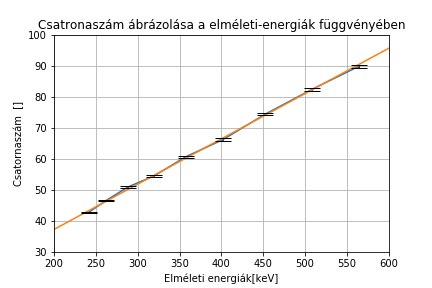
\includegraphics[width=1.\linewidth]{ch_en.png}
    \end{minipage}
\end{figure}

\par Itt az illesztett paraméterek értéke $a = (0.1458 \pm 0.00167) ~{1/keV}$, míg $b = (8.08748 \pm 0.5751)$. Ellenben, nekünk nem ezekre az adatokra, hanem ezek inverzére volt szükségünk így azokat véve, és a hibaterjedést figyelembe véve kapjuk, hogy

\begin{gather*}
	E = A x + B \\
	A = \frac{1}{a} = (6.857 \pm 0.079) ~keV \\
	B = -\frac{b}{a} = (-55.453 \pm 4.578) ~keV
\end{gather*}

\par Így kiszámolva a mért energiákat és azok hibáját

\begin{center}
\begin{tabular}{|c| c| c| c|}\hline
$\phi$ [$^{\circ}$] & $\text{elméleti energia}$ [keV] & $\text{mért energia}$ [keV] & $\chi^{2}$ \\ \hline
30 & 563.8223 & 559.7893&2.4760 \\ \hline
40 &507.7891 &508.8791&0.1938 \\ \hline
50 &452.3664 &454.4995&0.5390\\ \hline
60&401.5895 &398.0972&1.4060\\ \hline
70&357.2257 &360.2694&3.2993\\ \hline
80& 319.5971&318.1562&0.4012\\ \hline
90& 288.2794&293.6576&4.2930\\ \hline
100&262.5517 &264.2339&1.6734\\ \hline
110&241.6414 &238.0438&7.2402\\ \hline
\end{tabular}
\end{center}

\par Ekkor kiszámolva $\chi^{2}$-ek összegét erre nagyjából $21.5$-et kapunk. Az eredményt az alábbi képletbe helyettesítve számoltuk

\begin{equation*}
	\chi^{2} = \sum_{i}\frac{(E_{\text{mért}, i} - E_{\text{elméleti}, i} + \epsilon E_{\text{szisztematikus} , i})^{2}}{(\Delta E_{\text{mért,i}})^{2}}
\end{equation*}

\par Ahol az energia szisztematikus hibáját a kalibrációs egyenes illesztési hibájából számoltuk. A konfidencia szint a $(9-2)$ szabadsági fokú rendszerre ekkor $0.3\%$, aminek számításához a $scipy$ köyvtárat használtuk. Természetesen ezt az értéket $\epsilon = 0~$-nál vettük.

\begin{figure}[!htb]
\centering
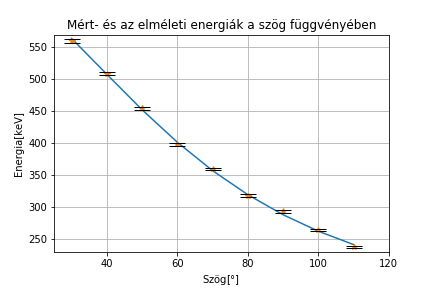
\includegraphics[width=0.86\textwidth]{en_deg.png}
\end{figure}

\subsection{Klein-Nishina formula vizsgálata}
\par Ehhez felhasználjuk az elméleti összefoglalóban említett képletet

\begin{equation*}
	\frac{d\sigma}{d\Omega} = \frac{1}{2}r_{0}^{2}(P - P^{2}sin^{2}\vartheta + P^{3})
\end{equation*}

\par Itt felhaználjük az illesztett Gauss-görbék területét, amelyet illesztési paraméterként megkaptunk. A laborhoz tartozó mérési leírásban szereplő képletek segítsével kiszámolható a hatásfok ($\eta$), valamint az $\frac{1}{\eta}\frac{dN}{dt}$ mennyiség, ami lényegében a differenciális hatáskeresztmetszek a $K$ állandóval leosztva. Az adatokat táblázatba foglalva

\begin{table}[h]
\begin{center}
\begin{tabular}{|c|c|c|c|c|c|}
\hline
szög[$^{\circ}$] &  $\eta$ & $\frac{1}{\eta}\frac{dN_{\text{mért}}}{dt}$ [$s^{-1}$] & $\Delta\left(\frac{
1}{\eta}\frac{dN_{\text{mért}}}{dt}\right)$ [$s^{-1}$] & illesztett függvény [$s^{-1}$]& $\chi^{2}$ \\
\hline
30 & 0.0974 & 1.39 & 0.10 & 1.34 & 0.27 \\
\hline
40 & 0.115 & 1.38 & 0.28 & 1.02 & 1.76 \\
\hline
50 & 0.140 & 0.859 & 0.089 & 0.779 & 0.79 \\
\hline
60 & 0.169 & 0.522 & 0.160 & 0.618 & 0.36 \\
\hline
70 & 0.200 & 0.460 & 0.063 & 0.511 & 0.66 \\
\hline
80 & 0.234 & 0.471 & 0.044 & 0.442 & 0.45 \\
\hline
90 & 0.267 & 0.381 & 0.069 & 0.397 & 0.05 \\
\hline
100 & 0.298 & 0.303 & 0.028 & 0.367 & 5.09 \\
\hline
110 & 0.327 & 0.391 & 0.034 & 0.348 & 1.61 \\
\hline
\end{tabular}
\end{center}
\end{table}

\par Hatásfok, hatásfokkal súlyozott beütési gyakoriság, valamint az arra illesztett függvény ($K\cdot (P-P^2\sin^2{\theta}+P^3)$) értékei és a hozzájuk tartozó $\chi^2$.

\begin{figure}[!htb]
\centering
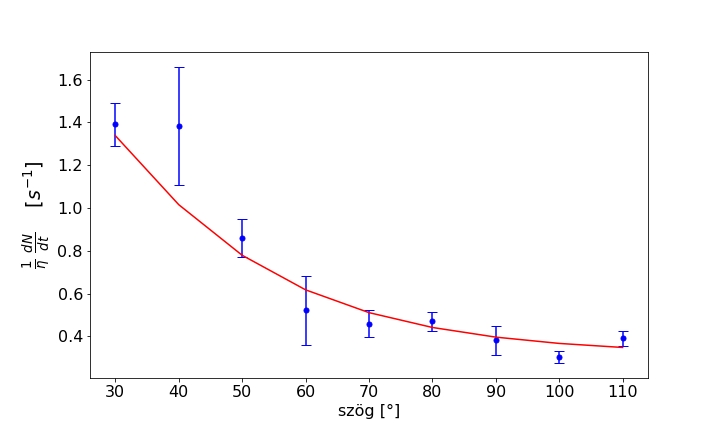
\includegraphics[width=0.86\textwidth]{../notebook/klein-nishina.png}
\end{figure}

\par Ahol $K = 2.26 10^{-26}~cm^{-2}s^{-1}$, a mérés leírásából lett véve. Esetünkben 9 szabadsági fokkal számolva a $\chi^{2}$-ek összege $11.04$ lett, ebből a konfidencia szint nagyjából $20\%$-os.

\section{Összefoglalás}
\par Úgy gondoljuk, hogy a konfidencia szinte jelentős mértékben növelhető volna, ha több ideig mérnénk egy-egy szögnél, hiszen ekkor a csúcsaink több beütést tartalmaznának és így a statisztikus hiba, valamint az illesztésből származó hiba csökkenthető lenne. Meglepődve tapasztaltuk, hogy ilyen alacsony konfidencia szintet sikerült csak produkálnunk, viszont a példa feladatok alapján megnyugodtunk, hiszen ott is csak $0,4\%$-os szint volt. Feltételezzük, hogy ennek elérése is komoly kiértékelési pontosságot követel meg, hiszen mi is próbáltunk a lehető legpontosabban eljárni a számolások, illesztések során. Így a mérés sikeresnek tekinthető.

\end{document}